%\documentclass[border=3pt,tikz]{standalone}
\documentclass[10pt,a4papper]{article}
\usepackage{graphicx}
\usepackage{amsmath}
\usepackage{amssymb}
\usepackage{tikz}
\usepackage{listofitems}
\usetikzlibrary{arrows.meta}
\usepackage[outline]{contour}
\usepackage{cancel}
\usepackage{multicol}
\usepackage{blindtext}
\usepackage[hidelinks]{hyperref}
\usepackage[left=2.00cm, right=3.00cm, top=2.00cm, bottom=2.00cm]{geometry}
\author{Angel Fdo. García Núñez}
\date{Enero 18, 2023}
\title{Estadisitica}

\tikzset{>=latex}
\usepackage{xcolor}
\colorlet{myred}{red!80!black}
\colorlet{myblue}{blue!80!black}
\colorlet{mygreen}{green!60!black}
\colorlet{myorange}{orange!70!red!60!black}
\colorlet{mydarkred}{red!30!black}
\colorlet{mydarkblue}{blue!40!black}
\colorlet{mydarkgreen}{green!30!black}
\tikzstyle{node}=[thick,circle,draw=myblue,minimum size=22,inner sep=0.5,outer sep=0.6]
\tikzstyle{node in}=[node,green!20!black,draw=mygreen!30!black,fill=mygreen!25]
\tikzstyle{node hidden}=[node,blue!20!black,draw=myblue!30!black,fill=myblue!20]
\tikzstyle{node convol}=[node,orange!20!black,draw=myorange!30!black,fill=myorange!20]
\tikzstyle{node out}=[node,red!20!black,draw=myred!30!black,fill=myred!20]
\tikzstyle{connect}=[thick,mydarkblue] %,line cap=round
\tikzstyle{connect arrow}=[-{Latex[length=4,width=3.5]},thick,mydarkblue,shorten <=0.5,shorten >=1]
\tikzset{
  node 1/.style={node in},
  node 2/.style={node hidden},
  node 3/.style={node out},
}
\def\nstyle{int(\lay<\Nnodlen?min(2,\lay):3)}

\begin{document}

\Huge
Clasificación de trazos de numéros

\Large
\newpage
\[\text{Dataset a clasificar}\]
\[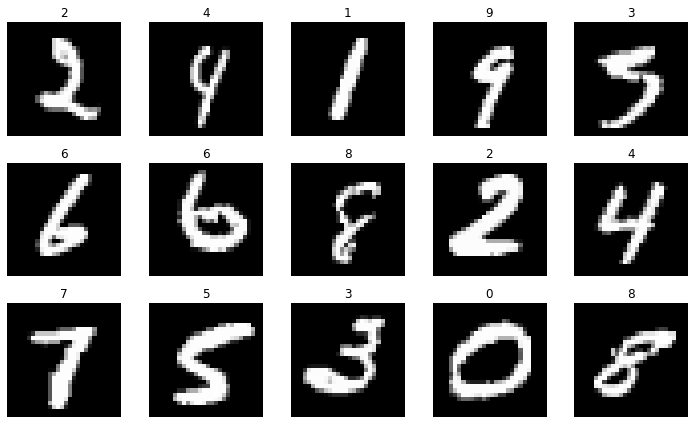
\includegraphics[height=10cm]{set.png}\]\\

Tenemos imágenes de 28x28 de un total de 784 píxeles, por lo que la entrada
de la red sera un vector de 784 componentes, y un total de 10 clases a clasificar
(números de $0-10$), así que la salida de la red sera un vector de 10
componentes:

\[\text{Capa de entrada $\vec x$ de 784 componentes}\]
\[\vec x=(x_1,x_2,x_3,...,x_{784})\]

\[\text{Capa oculta $\vec a$ de 100 componentes}\]
\[\vec a=(a_1,a_2,a_3,...,a_{100})\]

\[\text{Capa oculta $\vec y$ de 10 componentes}\]
\[\vec y=(y_1,y_2,y_3,y_4,y_5,y_6,y_7,y_8,y_9,y_{10})\]

\newpage
\[\text{Red Neuronal}\]

\begin{center}
  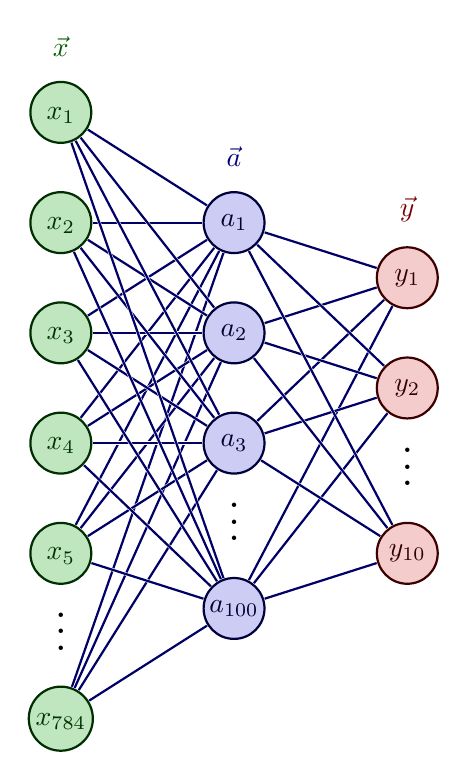
\begin{tikzpicture}[x=2.2cm,y=1.4cm]
    \message{^^JNeural network, shifted}
    \readlist\Nnod{6,4,3} % array of number of nodes per layer
    \readlist\Nstr{784,100,10} % array of string number of nodes per layer
    \readlist\Cstr{\strut x,a,y} % array of coefficient symbol per layer
    \def\yshift{0.5} % shift last node for dots
    
    \message{^^J  Layer}
    \foreachitem \N \in \Nnod{ % loop over layers
      \def\lay{\Ncnt} % alias of index of current layer
      \pgfmathsetmacro\prev{int(\Ncnt-1)} % number of previous layer
      \message{\lay,}
      \foreach \i [evaluate={\c=int(\i==\N); \y=\N/2-\i-\c*\yshift;
          \index=(\i<\N?int(\i):"\Nstr[\lay]");
          \x=\lay; \n=\nstyle;}] in {1,...,\N}{ % loop over nodes
        % NODES
        \node[node \n] (N\lay-\i) at (\x,\y) {$\Cstr[\lay]_{\index}$};
        
        % CONNECTIONS
        \ifnum\lay>1 % connect to previous layer
        \foreach \j in {1,...,\Nnod[\prev]}{ % loop over nodes in previous layer
          \draw[connect,white,line width=1.2] (N\prev-\j) -- (N\lay-\i);
          \draw[connect] (N\prev-\j) -- (N\lay-\i);
          %\draw[connect] (N\prev-\j.0) -- (N\lay-\i.180); % connect to left
        }
        \fi % else: nothing to connect first layer
        
      }
      \path (N\lay-\N) --++ (0,1+\yshift) node[midway,scale=1.5] {$\vdots$};
    }
    
    % LABELS
    \node[above=5,align=center,mygreen!60!black] at (N1-1.90) {$\vec x$};
    \node[above=5,align=center,myblue!60!black] at (N2-1.90) {$\vec a$};
    \node[above=5,align=center,myred!60!black] at (N\Nnodlen-1.90) {$\vec y$};
    
  \end{tikzpicture}
\end{center}

\[\text{Función de activación ReLU}\]

\[\varphi(s)=
\left\{\begin{array}{ccc}
s & : & s\geq 0\\
0 & : & s<0
\end{array}\]\\

\[\text{Comportamiento}\]

\[a_i=\varphi(\vec w_{a_i}\cdot\vec x+b_{a_i})\quad,\quad y_i=\varphi(\vec w_{y_i}\cdot\vec a+b_{y_i})\]\\

\[\text{Algoritmo de aprendizaje por retro-propagación}\]

\[\vec w_{j+1}=\vec w_j-\alpha\nabla E\quad,\quad
b_{j+1}=b_j-\alpha\nabla E\]


\newpage

\newpage

\newpage

\newpage

\newpage

\newpage

\newpage

\newpage

\newpage

\newpage

\newpage

\newpage

\newpage

\newpage

\newpage

\newpage

\newpage

\newpage

\newpage

\newpage

\newpage

\newpage

\newpage

\end{document}
